\documentclass[UTF8,10pt,aspectratio=169]{ctexbeamer}
\usepackage{amsmath, amssymb}
\usepackage{tikz}
\usetikzlibrary{calc}
\usepackage{newtxtext, newtxmath} % 经典试卷西文与公式字体

% 极简风格设置
\usetheme{default}
\usecolortheme{default}
\usefonttheme{serif} % 强制使用衬线体（宋体/Times风格），这是产生“试卷感”的关键
\setbeamertemplate{navigation symbols}{} % 去掉右下角导航图标
\setbeamertemplate{footline}[frame number] % 仅保留页码

\title{平面向量的线性运算}
\author{}
\date{}

\begin{document}
	
	\begin{frame}
		\titlepage
		\begin{center}
			{\Large \textbf{平面向量的线性运算}}
			
			\vspace{0.5cm}
			{\large 高一数学素养提升课学案（6）}
		\end{center}
	\end{frame}
	
	% ==================== 题目1 ====================
	\begin{frame}
		1.（2025·天津·高考真题）$\triangle ABC$ 中，$D$ 为 $AB$ 边中点，$\overrightarrow{CE} = \dfrac{1}{3}\overrightarrow{CD}$，$\overrightarrow{AB} = \vec{a}$，$\overrightarrow{AC} = \vec{b}$，则 $\overrightarrow{AE} = $ \underline{\hspace{2.5cm}}（用 $\vec{a}$，$\vec{b}$ 表示）。
		
		\vspace{0.3cm}
		\begin{center}
			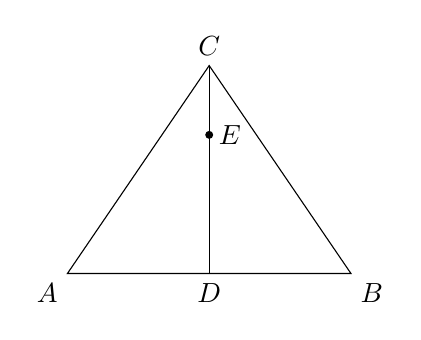
\begin{tikzpicture}[scale=1.2]
				\coordinate (A) at (0,0);
				\coordinate (B) at (3,0);
				\coordinate (C) at (1.5,2.2);
				\coordinate (D) at (1.5,0);
				\coordinate (E) at ($(C)!1/3!(D)$);
				\draw (A)--(B)--(C)--cycle;
				\draw (C)--(D);
				\fill (E) circle (1.2pt);
				\node[below left] at (A) {$A$};
				\node[below right] at (B) {$B$};
				\node[above] at (C) {$C$};
				\node[below] at (D) {$D$};
				\node[right] at (E) {$E$};
			\end{tikzpicture}
		\end{center}
		
		\pause
		\textbf{【答案】} $\dfrac{1}{6}\vec{a} + \dfrac{2}{3}\vec{b}$
		
		\vspace{0.2cm}
		\textbf{【详解】} 
		$\overrightarrow{AE} = \overrightarrow{AC} + \overrightarrow{CE} = \overrightarrow{AC} + \dfrac{1}{3}\overrightarrow{CD} = \overrightarrow{AC} + \dfrac{1}{3}(\overrightarrow{AD} - \overrightarrow{AC})$
		
		\vspace{0.1cm}
		$= \dfrac{2}{3}\overrightarrow{AC} + \dfrac{1}{3}\overrightarrow{AD} = \dfrac{2}{3}\vec{b} + \dfrac{1}{3} \cdot \dfrac{1}{2}\vec{a} = \dfrac{1}{6}\vec{a} + \dfrac{2}{3}\vec{b}$。
	\end{frame}
	
	% ==================== 题目2 ====================
	\begin{frame}
		2.（2020·山东·高考真题）已知平行四边形 $ABCD$，点 $E$，$F$ 分别是 $AB$，$BC$ 的中点（如图所示）。设 $\overrightarrow{AB} = \vec{a}$，$\overrightarrow{AD} = \vec{b}$，则 $\overrightarrow{EF}$ 等于（\quad）
		
		\vspace{0.2cm}
		\begin{center}
			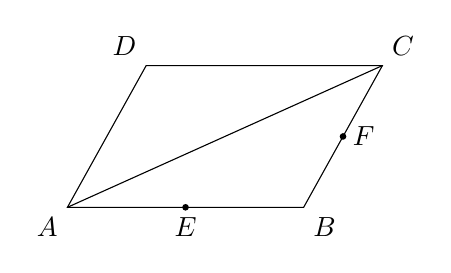
\begin{tikzpicture}[scale=1.0]
				\coordinate (A) at (0,0);
				\coordinate (B) at (3,0);
				\coordinate (C) at (4,1.8);
				\coordinate (D) at (1,1.8);
				\coordinate (E) at ($(A)!0.5!(B)$);
				\coordinate (F) at ($(B)!0.5!(C)$);
				\draw (A)--(B)--(C)--(D)--cycle;
				\draw (A)--(C);
				\node[below left] at (A) {$A$};
				\node[below right] at (B) {$B$};
				\node[above right] at (C) {$C$};
				\node[above left] at (D) {$D$};
				\node[below] at (E) {$E$};
				\node[right] at (F) {$F$};
				\fill (E) circle (1.2pt);
				\fill (F) circle (1.2pt);
			\end{tikzpicture}
		\end{center}
		
		\vspace{0.2cm}
		A. $\dfrac{1}{2}(\vec{a} + \vec{b})$ \quad B. $\dfrac{1}{2}(\vec{a} - \vec{b})$ \quad C. $\dfrac{1}{2}(\vec{b} - \vec{a})$ \quad D. $\dfrac{1}{2}\vec{a} + \vec{b}$
		
		\pause
		\vspace{0.2cm}
		\textbf{【答案】} A
		
		\vspace{0.1cm}
		\textbf{【详解】} 在 $\triangle ABC$ 中，$E$，$F$ 分别为 $AB$，$BC$ 的中点，由三角形中位线（或向量运算）：
		$$\overrightarrow{EF} = \dfrac{1}{2}\overrightarrow{AC} = \dfrac{1}{2}(\overrightarrow{AB} + \overrightarrow{AD}) = \dfrac{1}{2}(\vec{a} + \vec{b})。$$
	\end{frame}
	
	% ==================== 题目3 ====================
	\begin{frame}
		3.（2018·全国 I 卷·高考真题）在 $\triangle ABC$ 中，$AD$ 为 $BC$ 边上的中线，$E$ 为 $AD$ 的中点，则 $\overrightarrow{EB} = $（\quad）
		
		\vspace{0.2cm}
		\begin{center}
			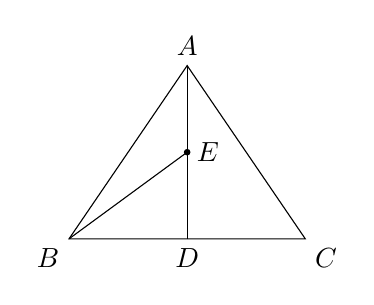
\begin{tikzpicture}[scale=1.0]
				\coordinate (A) at (1.5,2.2);
				\coordinate (B) at (0,0);
				\coordinate (C) at (3,0);
				\coordinate (D) at ($(B)!0.5!(C)$);
				\coordinate (E) at ($(A)!0.5!(D)$);
				\draw (A)--(B)--(C)--cycle;
				\draw (A)--(D);
				\draw (B)--(E);
				\fill (E) circle (1.2pt);
				\node[above] at (A) {$A$};
				\node[below left] at (B) {$B$};
				\node[below right] at (C) {$C$};
				\node[below] at (D) {$D$};
				\node[right] at (E) {$E$};
			\end{tikzpicture}
		\end{center}
		
		\vspace{0.1cm}
		A. $\dfrac{3}{4}\overrightarrow{AB} - \dfrac{1}{4}\overrightarrow{AC}$ \qquad B. $\dfrac{1}{4}\overrightarrow{AB} - \dfrac{3}{4}\overrightarrow{AC}$
		
		\vspace{0.1cm}
		C. $\dfrac{3}{4}\overrightarrow{AB} + \dfrac{1}{4}\overrightarrow{AC}$ \qquad D. $\dfrac{1}{4}\overrightarrow{AB} + \dfrac{3}{4}\overrightarrow{AC}$
		
		\pause
		\vspace{0.2cm}
		\textbf{【答案】} A
		
		\vspace{0.1cm}
		\textbf{【详解】} $\overrightarrow{AD} = \dfrac{1}{2}(\overrightarrow{AB} + \overrightarrow{AC})$，$\overrightarrow{AE} = \dfrac{1}{2}\overrightarrow{AD} = \dfrac{1}{4}\overrightarrow{AB} + \dfrac{1}{4}\overrightarrow{AC}$，
		
		\vspace{0.1cm}
		故 $\overrightarrow{EB} = \overrightarrow{AB} - \overrightarrow{AE} = \overrightarrow{AB} - \dfrac{1}{4}\overrightarrow{AB} - \dfrac{1}{4}\overrightarrow{AC} = \dfrac{3}{4}\overrightarrow{AB} - \dfrac{1}{4}\overrightarrow{AC}$。
	\end{frame}
	
	% ==================== 题目4 ====================
	\begin{frame}
		4. 设 $\vec{a}$，$\vec{b}$ 是两个不共线的向量，$\overrightarrow{AB} = 2\vec{a} + k\vec{b}$，$\overrightarrow{BC} = \vec{a} + \vec{b}$，$\overrightarrow{CD} = \vec{a} - 2\vec{b}$，若 $A$，$B$，$D$ 三点共线，则实数 $k$ 的值为 \underline{\hspace{2cm}}。
		
		\pause
		\vspace{0.3cm}
		\textbf{【答案】} $k = -1$
		
		\vspace{0.2cm}
		\textbf{【详解】} 由已知：
		$$\overrightarrow{BD} = \overrightarrow{BC} + \overrightarrow{CD} = (\vec{a} + \vec{b}) + (\vec{a} - 2\vec{b}) = 2\vec{a} - \vec{b}。$$
		
		\vspace{0.1cm}
		因为 $A$，$B$，$D$ 三点共线，所以 $\overrightarrow{AB} \parallel \overrightarrow{BD}$，即存在实数 $\lambda$，使得 $\overrightarrow{AB} = \lambda \overrightarrow{BD}$。
		
		\vspace{0.1cm}
		即 $2\vec{a} + k\vec{b} = \lambda(2\vec{a} - \vec{b}) = 2\lambda\vec{a} - \lambda\vec{b}$。
		
		\vspace{0.1cm}
		由 $\vec{a}$，$\vec{b}$ 不共线，故 $\begin{cases} 2 = 2\lambda \\ k = -\lambda \end{cases}$，解得 $\lambda = 1$，$k = -1$。
	\end{frame}
	
	% ==================== 题目5(1) ====================
	\begin{frame}
		5.(1) 如图 1，$A$，$B$，$C$ 是平面内的三个点，且 $A$ 与 $B$ 不重合，$P$ 是平面内任意一点，若点 $C$ 在直线 $AB$ 上，试证明：存在实数 $\lambda$，使得：
		$$\overrightarrow{PC} = \lambda \overrightarrow{PA} + (1 - \lambda)\overrightarrow{PB}。$$
		
		\vspace{0.2cm}
		\begin{center}
			\begin{tikzpicture}[scale=1.0]
				\coordinate (A) at (1,1.8);
				\coordinate (B) at (3.5,1.5);
				\coordinate (C) at (2.5,1.62);
				\coordinate (P) at (0,0);
				\draw[dashed] (A)--(B);
				\draw[dashed] (P)--(A);
				\draw[dashed] (P)--(B);
				\draw[dashed] (P)--(C);
				\fill (A) circle (1.2pt);
				\fill (B) circle (1.2pt);
				\fill (C) circle (1.2pt);
				\fill (P) circle (1.2pt);
				\node[above] at (A) {$A$};
				\node[right] at (B) {$B$};
				\node[above] at (C) {$C$};
				\node[left] at (P) {$P$};
				\node at (2,-0.3) {图 1};
			\end{tikzpicture}
		\end{center}
		
		\pause
		\textbf{【证明】} 因为 $C$ 在直线 $AB$ 上，所以 $\overrightarrow{AC} \parallel \overrightarrow{AB}$，故存在实数 $t$，使得 $\overrightarrow{AC} = t\overrightarrow{AB}$。
		
		\vspace{0.1cm}
		即 $\overrightarrow{PC} - \overrightarrow{PA} = t(\overrightarrow{PB} - \overrightarrow{PA})$，整理得：
		$$\overrightarrow{PC} = (1-t)\overrightarrow{PA} + t\overrightarrow{PB}。$$
		令 $\lambda = 1 - t$，则 $\overrightarrow{PC} = \lambda \overrightarrow{PA} + (1-\lambda)\overrightarrow{PB}$，证毕。
	\end{frame}
	
	% ==================== 题目5(2) ====================
	\begin{frame}
		5.(2) 如图 2，设 $G$ 为 $\triangle ABC$ 的重心，$PQ$ 过 $G$ 点且与 $AB$、$AC$（或其延长线）分别交于 $P$，$Q$ 点，若 $\overrightarrow{AP} = m\overrightarrow{AB}$，$\overrightarrow{AQ} = n\overrightarrow{AC}$，试探究 $\dfrac{1}{m} + \dfrac{1}{n}$ 的值是否为定值，若为定值，求出这个定值；若不是定值，请说明理由。
		
		\vspace{0.2cm}
		\begin{center}
			\begin{tikzpicture}[scale=1.0]
				\coordinate (A) at (2,2.4);
				\coordinate (B) at (0,0);
				\coordinate (C) at (4,0);
				\coordinate (M) at ($(B)!0.5!(C)$);
				\coordinate (G) at ($(A)!2/3!(M)$);
				\coordinate (P) at ($(A)!1.3!(B)$);
				\coordinate (Q) at ($(A)!0.8!(C)$);
				\draw (A)--(B)--(C)--cycle;
				\draw[dashed] (A)--(M);
				\draw (P)--(Q);
				\fill (G) circle (1.2pt);
				\fill (M) circle (1pt);
				\node[above] at (A) {$A$};
				\node[below left] at (B) {$B$};
				\node[below right] at (C) {$C$};
				\node[below] at (M) {$M$};
				\node[above right] at (G) {$G$};
				\node[left] at (P) {$P$};
				\node[right] at (Q) {$Q$};
				\node at (2,-0.8) {图 2};
			\end{tikzpicture}
		\end{center}
		
		\pause
		\textbf{【答案】} $\dfrac{1}{m} + \dfrac{1}{n} = 3$（定值）。
	\end{frame}
	
	% ==================== 题目5(2) 详解 ====================
	\begin{frame}
		\textbf{【详解】} 设 $M$ 为 $BC$ 中点，因为 $G$ 为 $\triangle ABC$ 的重心，所以：
		$$\overrightarrow{AG} = \dfrac{2}{3}\overrightarrow{AM} = \dfrac{2}{3} \cdot \dfrac{1}{2}(\overrightarrow{AB} + \overrightarrow{AC}) = \dfrac{1}{3}\overrightarrow{AB} + \dfrac{1}{3}\overrightarrow{AC}。$$
		
		\vspace{0.2cm}
		又因 $\overrightarrow{AP} = m\overrightarrow{AB}$，$\overrightarrow{AQ} = n\overrightarrow{AC}$，即 $\overrightarrow{AB} = \dfrac{1}{m}\overrightarrow{AP}$，$\overrightarrow{AC} = \dfrac{1}{n}\overrightarrow{AQ}$，
		
		\vspace{0.1cm}
		代入得：
		$$\overrightarrow{AG} = \dfrac{1}{3m}\overrightarrow{AP} + \dfrac{1}{3n}\overrightarrow{AQ}。$$
		
		\vspace{0.2cm}
		由于 $P$，$G$，$Q$ 三点共线（由第(1)题结论），所以系数之和为 $1$：
		$$\dfrac{1}{3m} + \dfrac{1}{3n} = 1，\quad \text{即 } \dfrac{1}{m} + \dfrac{1}{n} = 3。$$
		
		故 $\dfrac{1}{m} + \dfrac{1}{n}$ 为定值 $3$。
	\end{frame}
	
	% ==================== 归纳提升：三点共线定理 ====================
	\begin{frame}
		\begin{center}
			{\Large \textbf{归纳提升：三点共线的向量表示}}
		\end{center}
		\vspace{0.4cm}
		
		\textbf{1. 三点共线定理} \\
		设 $A$，$B$，$C$ 是平面内三点（$A$，$B$ 不重合），$P$ 为平面内任意一点，则：
		$$A, B, C \text{ 三点共线} \iff \exists\, \lambda \in \mathbb{R},\ \overrightarrow{PC} = \lambda \overrightarrow{PA} + (1-\lambda)\overrightarrow{PB}。$$
		
		\pause
		\vspace{0.3cm}
		\textbf{2. 等价刻画（系数和为 1）} \\
		若 $\overrightarrow{PC} = x\overrightarrow{PA} + y\overrightarrow{PB}$，则：
		$$A, B, C \text{ 三点共线} \iff x + y = 1。$$
		
		\pause
		\vspace{0.3cm}
		\textbf{3. 解题要点} 
		\begin{itemize}
			\item \textbf{结构识别}：题中出现三点共线条件，优先设法写出其中一点相对另一点的线性组合，利用“系数和为 1”建立方程。
			\item \textbf{常见应用}：求参数值（如第 4 题）、证明定值问题（如第 5(2) 题）。
		\end{itemize}
	\end{frame}
	
	% ==================== 归纳提升：系数与点的位置关系 ====================
	\begin{frame}
		\begin{center}
			{\Large \textbf{深入探究：系数 $\lambda$、$\mu$ 的取值与点 $C$ 的位置}}
		\end{center}
		\vspace{0.3cm}
		
		设 $\overrightarrow{PC} = \lambda \overrightarrow{PA} + \mu \overrightarrow{PB}$，$\lambda + \mu = 1$。变形可得：
		$$\overrightarrow{PC} - \overrightarrow{PB} = \lambda(\overrightarrow{PA} - \overrightarrow{PB}) \implies \overrightarrow{BC} = \lambda \overrightarrow{BA}。$$
		
		\vspace{0.2cm}
		即 \textbf{$\lambda$ 就是 $\overrightarrow{BC}$ 关于 $\overrightarrow{BA}$ 的比例系数}；同理 $\overrightarrow{AC} = \mu \overrightarrow{AB}$。
		
		\pause
		\vspace{0.3cm}
		\textbf{分类讨论}（设 $A$、$B$ 不重合，$C$ 在直线 $AB$ 上）：
		
		\vspace{0.2cm}
		\begin{center}
			\renewcommand{\arraystretch}{1.3}
			\begin{tabular}{|c|c|c|}
				\hline
				\textbf{$C$ 的位置} & \textbf{$\lambda$（$A$ 的系数）} & \textbf{$\mu$（$B$ 的系数）} \\
				\hline
				$C = A$ & $1$ & $0$ \\
				\hline
				$C = B$ & $0$ & $1$ \\
				\hline
				$C$ 为 $AB$ 中点 & $\dfrac{1}{2}$ & $\dfrac{1}{2}$ \\
				\hline
				$C$ 在线段 $AB$ 内部 & $0 < \lambda < 1$ & $0 < \mu < 1$ \\
				\hline
				$C$ 在 $BA$ 延长线上（$A$ 外侧） & $\lambda > 1$ & $\mu < 0$ \\
				\hline
				$C$ 在 $AB$ 延长线上（$B$ 外侧） & $\lambda < 0$ & $\mu > 1$ \\
				\hline
			\end{tabular}
		\end{center}
	\end{frame}
	
	% ==================== 归纳提升：直观记忆与推广 ====================
	\begin{frame}
		\begin{center}
			{\Large \textbf{直观记忆口诀与推广}}
		\end{center}
		\vspace{0.3cm}
		
		\textbf{1. 记忆口诀}
		\begin{itemize}
			\item \textbf{“离谁近，谁的系数大”}：$C$ 靠近 $A$，则 $\lambda$ 大；$C$ 靠近 $B$，则 $\mu$ 大。
			\item \textbf{“跑外侧，对侧系数变负”}：$C$ 跑到 $A$ 外侧，$B$ 的系数 $\mu$ 变负；反之亦然。
		\end{itemize}
		
		\pause
		\vspace{0.4cm}
		\textbf{2. 推广：系数和 $\neq 1$ 的情形} \\
		若 $\overrightarrow{OC} = x\overrightarrow{OA} + y\overrightarrow{OB}$（$O$ 为任意一点），记 $k = x + y$：
		\begin{itemize}
			\item $k = 1$：$C$ 在直线 $AB$ 上；
			\item $0 < k < 1$：$C$ 在直线 $AB$ 靠近 $O$ 的一侧；
			\item $k > 1$：$C$ 在直线 $AB$ 远离 $O$ 的一侧；
			\item $x > 0$，$y > 0$ 且 $x + y < 1$：$C$ 在 $\triangle OAB$ \textbf{内部}。
		\end{itemize}
		
		\pause
		\vspace{0.3cm}
		\textbf{3. 应用提醒} \\
		在处理“重心”“内心”“三角形内点的向量表示”等问题时，
		若题设中 $\lambda$、$\mu$ 带有正负限制（如 $\lambda > 0$），往往隐含了点的位置约束，需结合几何图形验证。
	\end{frame}
	
	% ==================== 题目6(1) ====================
	\begin{frame}
		6.（2025 山东济南师范大学附属中学月考）如图，在 $\triangle ABC$ 中，点 $P$ 满足 $\overrightarrow{PC} = 2\overrightarrow{BP}$，$O$ 是线段 $AP$ 的中点，过点 $O$ 的直线与边 $AB$，$AC$ 分别交于点 $E$，$F$。
		
		\vspace{0.2cm}
		(1) 若 $\overrightarrow{AF} = \dfrac{2}{3}\overrightarrow{AC}$，求 $\dfrac{AE}{EB}$ 的值；
		
		\vspace{0.2cm}
		\begin{center}
			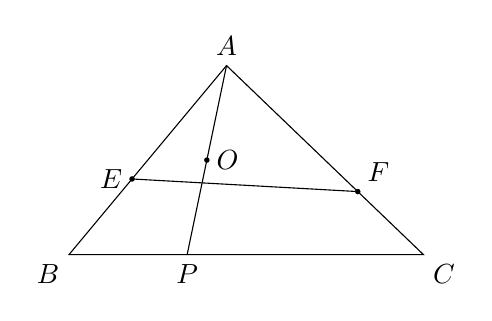
\begin{tikzpicture}[scale=1.0]
				\coordinate (A) at (2,2.4);
				\coordinate (B) at (0,0);
				\coordinate (C) at (4.5,0);
				\coordinate (P) at ($(B)!1/3!(C)$);
				\coordinate (O) at ($(A)!0.5!(P)$);
				\coordinate (E) at ($(A)!0.6!(B)$);
				\coordinate (F) at ($(A)!2/3!(C)$);
				\draw (A)--(B)--(C)--cycle;
				\draw (A)--(P);
				\draw (E)--(F);
				\fill (O) circle (1pt);
				\fill (E) circle (1pt);
				\fill (F) circle (1pt);
				\node[above] at (A) {$A$};
				\node[below left] at (B) {$B$};
				\node[below right] at (C) {$C$};
				\node[below] at (P) {$P$};
				\node[right] at (O) {$O$};
				\node[left] at (E) {$E$};
				\node[above right] at (F) {$F$};
			\end{tikzpicture}
		\end{center}
		
		\pause
		\textbf{【答案】} $\dfrac{AE}{EB} = \dfrac{4}{5}$
	\end{frame}
	
	% ==================== 题目6(1) 详解 ====================
	\begin{frame}
		\textbf{【详解】} 由 $\overrightarrow{PC} = 2\overrightarrow{BP}$ 知 $P$ 是 $BC$ 的三等分点（靠近 $B$），即 $\overrightarrow{BP} = \dfrac{1}{3}\overrightarrow{BC}$，
		
		\vspace{0.1cm}
		所以 $\overrightarrow{AP} = \overrightarrow{AB} + \overrightarrow{BP} = \overrightarrow{AB} + \dfrac{1}{3}(\overrightarrow{AC} - \overrightarrow{AB}) = \dfrac{2}{3}\overrightarrow{AB} + \dfrac{1}{3}\overrightarrow{AC}$。
		
		\vspace{0.2cm}
		$O$ 为 $AP$ 中点，故 $\overrightarrow{AO} = \dfrac{1}{2}\overrightarrow{AP} = \dfrac{1}{3}\overrightarrow{AB} + \dfrac{1}{6}\overrightarrow{AC}$。
		
		\vspace{0.2cm}
		设 $\overrightarrow{AE} = k\overrightarrow{AB}$，已知 $\overrightarrow{AF} = \dfrac{2}{3}\overrightarrow{AC}$，即 $\overrightarrow{AB} = \dfrac{1}{k}\overrightarrow{AE}$，$\overrightarrow{AC} = \dfrac{3}{2}\overrightarrow{AF}$。
		
		\vspace{0.1cm}
		代入得：$\overrightarrow{AO} = \dfrac{1}{3k}\overrightarrow{AE} + \dfrac{1}{6} \cdot \dfrac{3}{2}\overrightarrow{AF} = \dfrac{1}{3k}\overrightarrow{AE} + \dfrac{1}{4}\overrightarrow{AF}$。
		
		\vspace{0.2cm}
		由 $E$，$O$，$F$ 三点共线，系数和为 $1$：
		$$\dfrac{1}{3k} + \dfrac{1}{4} = 1 \implies \dfrac{1}{3k} = \dfrac{3}{4} \implies k = \dfrac{4}{9}。$$
		
		故 $AE = \dfrac{4}{9}AB$，$EB = \dfrac{5}{9}AB$，所以 $\dfrac{AE}{EB} = \dfrac{4}{5}$。
	\end{frame}
	
	% ==================== 题目6(2) ====================
	\begin{frame}
		6.(2) 若 $\overrightarrow{EB} = \lambda \overrightarrow{AE}\ (\lambda > 0)$，$\overrightarrow{FC} = \mu \overrightarrow{AF}\ (\mu > 0)$，求 $\dfrac{1}{\lambda} + \dfrac{1}{\mu + 1}$ 的最小值。
		
		\vspace{0.4cm}
		\textbf{【思路提示】} \ 基本不等式 $+$ “1” 的妙用。
		
		\pause
		\vspace{0.4cm}
		\textbf{【详解】} 由 $\overrightarrow{EB} = \lambda \overrightarrow{AE}$ 得 $\overrightarrow{AB} - \overrightarrow{AE} = \lambda \overrightarrow{AE}$，即 $\overrightarrow{AE} = \dfrac{1}{1+\lambda}\overrightarrow{AB}$。
		
		\vspace{0.1cm}
		由 $\overrightarrow{FC} = \mu \overrightarrow{AF}$ 得 $\overrightarrow{AC} - \overrightarrow{AF} = \mu \overrightarrow{AF}$，即 $\overrightarrow{AF} = \dfrac{1}{1+\mu}\overrightarrow{AC}$。
		
		\vspace{0.2cm}
		由上一题，$\overrightarrow{AO} = \dfrac{1}{3}\overrightarrow{AB} + \dfrac{1}{6}\overrightarrow{AC} = \dfrac{1+\lambda}{3}\overrightarrow{AE} + \dfrac{1+\mu}{6}\overrightarrow{AF}$。
		
		\vspace{0.2cm}
		由 $E$，$O$，$F$ 三点共线：
		$$\dfrac{1+\lambda}{3} + \dfrac{1+\mu}{6} = 1 \implies 2(1+\lambda) + (1+\mu) = 6 \implies 2\lambda + \mu = 3。$$
	\end{frame}
	
	% ==================== 题目6(2) 续 ====================
	\begin{frame}
		\textbf{【详解（续）】} 即约束条件为 $2\lambda + (\mu + 1) = 4$，其中 $\lambda > 0$，$\mu + 1 > 1 > 0$。
		
		\vspace{0.3cm}
		利用 “1” 的妙用：
		$$\dfrac{1}{\lambda} + \dfrac{1}{\mu + 1} = \dfrac{1}{4}\left[2\lambda + (\mu+1)\right]\left(\dfrac{1}{\lambda} + \dfrac{1}{\mu+1}\right)$$
		
		\vspace{0.1cm}
		$$= \dfrac{1}{4}\left[2 + 1 + \dfrac{\mu+1}{\lambda} + \dfrac{2\lambda}{\mu+1}\right] = \dfrac{1}{4}\left[3 + \dfrac{\mu+1}{\lambda} + \dfrac{2\lambda}{\mu+1}\right]。$$
		
		\vspace{0.2cm}
		由基本不等式：
		$$\dfrac{\mu+1}{\lambda} + \dfrac{2\lambda}{\mu+1} \geq 2\sqrt{\dfrac{\mu+1}{\lambda} \cdot \dfrac{2\lambda}{\mu+1}} = 2\sqrt{2}。$$
		
		\vspace{0.2cm}
		所以 $\dfrac{1}{\lambda} + \dfrac{1}{\mu + 1} \geq \dfrac{3 + 2\sqrt{2}}{4}$。
		
		\vspace{0.1cm}
		当且仅当 $\dfrac{\mu+1}{\lambda} = \dfrac{2\lambda}{\mu+1}$，即 $\mu + 1 = \sqrt{2}\lambda$ 时取等号，结合 $2\lambda + (\mu+1) = 4$ 可解得 $\lambda$，$\mu$ 的具体值。
		
		\vspace{0.2cm}
		故 $\dfrac{1}{\lambda} + \dfrac{1}{\mu + 1}$ 的最小值为 $\boxed{\dfrac{3 + 2\sqrt{2}}{4}}$。
	\end{frame}
	
\end{document}